%%%%%%%%%%%%%%%%%%%%%%%%%%%%%%%%%%%%%%%%%
% Journal Article
% LaTeX Template
% Version 1.4 (15/5/16)
%
% This template has been downloaded from:
% http://www.LaTeXTemplates.com
%
% Original author:
% Frits Wenneker (http://www.howtotex.com) with extensive modifications by
% Vel (vel@LaTeXTemplates.com)
%
% License:
% CC BY-NC-SA 3.0 (http://creativecommons.org/licenses/by-nc-sa/3.0/)
%
%%%%%%%%%%%%%%%%%%%%%%%%%%%%%%%%%%%%%%%%%

%----------------------------------------------------------------------------------------
%	PACKAGES AND OTHER DOCUMENT CONFIGURATIONS
%----------------------------------------------------------------------------------------

\documentclass[twoside,twocolumn]{article}

\usepackage{blindtext} % Package to generate dummy text throughout this template

\usepackage[sc]{mathpazo} % Use the Palatino font
\usepackage[T1]{fontenc} % Use 8-bit encoding that has 256 glyphs
\linespread{1.05} % Line spacing - Palatino needs more space between lines
\usepackage{microtype} % Slightly tweak font spacing for aesthetics

\usepackage[english]{babel} % Language hyphenation and typographical rules

\usepackage[hmarginratio=1:1,top=32mm,columnsep=20pt]{geometry} % Document margins
\usepackage[hang, small,labelfont=bf,up,textfont=it,up]{caption} % Custom captions under/above floats in tables or figures
\usepackage{booktabs} % Horizontal rules in tables

\usepackage{lettrine} % The lettrine is the first enlarged letter at the beginning of the text

\usepackage{enumitem} % Customized lists
\setlist[itemize]{noitemsep} % Make itemize lists more compact

\usepackage{abstract} % Allows abstract customization
\renewcommand{\abstractnamefont}{\normalfont\bfseries} % Set the "Abstract" text to bold
\renewcommand{\abstracttextfont}{\normalfont\small\itshape} % Set the abstract itself to small italic text

\usepackage{titlesec} % Allows customization of titles
\renewcommand\thesection{\Roman{section}} % Roman numerals for the sections
\renewcommand\thesubsection{\roman{subsection}} % roman numerals for subsections
\titleformat{\section}[block]{\large\scshape\centering}{\thesection.}{1em}{} % Change the look of the section titles
\titleformat{\subsection}[block]{\large}{\thesubsection.}{1em}{} % Change the look of the section titles

\usepackage{fancyhdr} % Headers and footers
\pagestyle{fancy} % All pages have headers and footers
\fancyhead{} % Blank out the default header
\fancyfoot{} % Blank out the default footer
\fancyhead[C]{} % Custom header text
\fancyfoot[RO,LE]{\thepage} % Custom footer text

\usepackage{titling} % Customizing the title section

\usepackage{hyperref} % For hyperlinks in the PDF

\usepackage{amsmath}
\newcommand*\diff{\mathop{}\!\mathrm{d}}
\newcommand*\Diff[1]{\mathop{}\!\mathrm{d^#1}}

\usepackage{graphicx}
\graphicspath{ {./images/} }

%----------------------------------------------------------------------------------------
%	TITLE SECTION
%----------------------------------------------------------------------------------------

\setlength{\droptitle}{-4\baselineskip} % Move the title up

\pretitle{\begin{center}\Huge\bfseries} % Article title formatting
\posttitle{\end{center}} % Article title closing formatting
\title{Scoring and Rewarding} % Article title
\author{%
\textsc{Parami Devs} % Your name
\normalsize \href{mailto:devs@parami.io}{devs@parami.io} % Your email address
%\and % Uncomment if 2 authors are required, duplicate these 4 lines if more
%\textsc{Jane Smith}\thanks{Corresponding author} \\[1ex] % Second author's name
%\normalsize University of Utah \\ % Second author's institution
%\normalsize \href{mailto:jane@smith.com}{jane@smith.com} % Second author's email address
}
\date{\today} % Leave empty to omit a date
\renewcommand{\maketitlehookd}{%
\begin{abstract}
\noindent We design and implement scoring and rewarding algorithms to help building
auditable, reliable, reusable decentralized profiles\cite{ref1} to drive
the de-authoritative advertisement network.

\end{abstract}
}

%----------------------------------------------------------------------------------------

\begin{document}

% Print the title
\maketitle

%----------------------------------------------------------------------------------------
%	ARTICLE CONTENTS
%----------------------------------------------------------------------------------------

\section{Introduction}

\lettrine[nindent=0em,lines=3]{S}coring and rewarding is the cornerstone of Parami Protocol.
The scoring algorithm is the key function to avoid fraud and spamming in the AD3 network.
Where it provides nonintrusive universal unique decentralized identifier.
People can earn rewards from advertiser directly by using their decentralized profile.

%------------------------------------------------

\section{Goals}

With the design of Parami Protocol, the goals of the scoring and rewarding algorithm are:
\begin{itemize}
    \item Data should be shared with peers in decentralized way
    \item Show every score activity is based on payment
    \item Reward identifier based on scores when advertiser confirms
    \item Smurfs should have low scores
    \item Detect dummy identifiers
\end{itemize}

% Text requiring further explanation\footnote{Example footnote}.

%------------------------------------------------

\section{Implementation}

\subsection{PCAP}

\begin{table}
    \centering
    \begin{tabular}{llr}
        \toprule
        Tag      & Score \\
        \midrule
        Telegram & $5$   \\
        Ethereum & $2$   \\
        Kusama   & $7$   \\
        \bottomrule
    \end{tabular}
    \caption{Example decrypted PCAP}
    \label{table:examplePCAP}
\end{table}

The Personal Crypto Advertising Preference (PCAP) ~\ref{table:examplePCAP} \cite{ref2}
provides an auditable and reliable way to store scores of an identifier.

An identifier can have multiple tags, each tag gets a score between -100 and 100.

To protect privacy, currently, a tag is hashed and stored opaquely.
The half-opaque profile will be moved to full-encrypted PCAP in the near term
by using the Paillier\cite{ref3} Homomorphic Encryption and Zero-Knowledge Proof scheme.

\subsection{On-Chain Scoring}

\begin{figure}
    \centering
    \begin{minipage}{.22\textwidth}
        \centering
        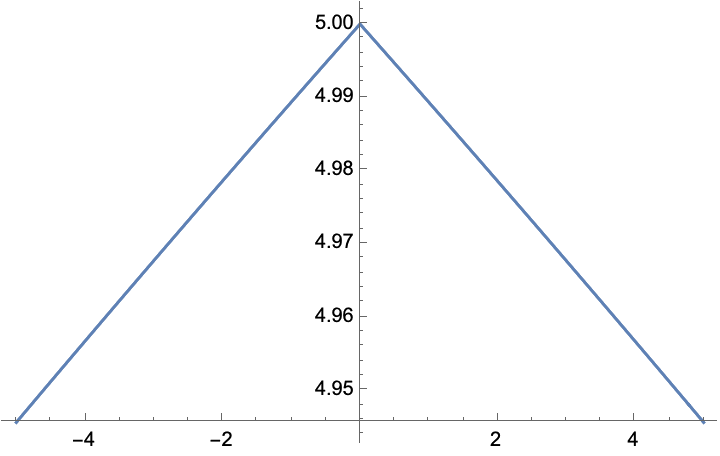
\includegraphics[width=0.8\textwidth]{scoring_p}
    \end{minipage}%
    \begin{minipage}{.22\textwidth}
        \centering
        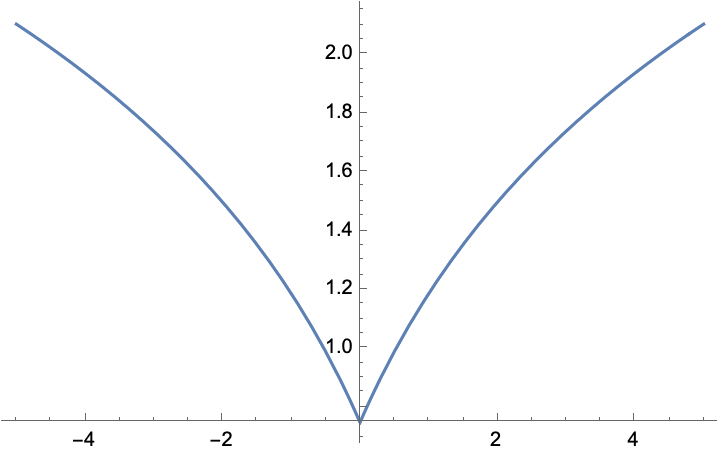
\includegraphics[width=0.8\textwidth]{scoring_n}
    \end{minipage}
    \captionof{figure}{s'' curve at ds=5}
    \label{fig:scoring_d}
\end{figure}

\begin{figure}
    \centering
    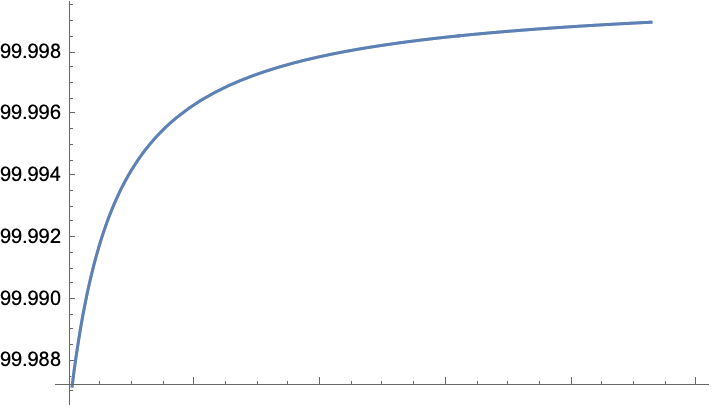
\includegraphics[width=0.3\textwidth]{score}
    \captionof{figure}{scoring curve}
    \label{fig:scoring}
\end{figure}

To prevent scores from fraud, the On-Chain Scoring algorithm is designed as a nonlinear function ~\ref{fig:scoring_d},
\begin{align*}
    {s}''=\left\{\begin{matrix}
                     \Delta\,s*log_{102}(102-|s|) & \cdots\,s*\Delta\,s\geq0 \\
                     \Delta\,s*log_{102}(|s|+2)   & \cdots\,s*\Delta\,s<0
                 \end{matrix}\right.
\end{align*}

it takes as input $-100<\Delta\,s<100$ and updates the state as follows:
\[
    (s)\mathop{\to}^{\Delta\,s}({s}')
\]

It is obvious that solution of the formula is on the interval (-100, 100).

\subsection{Rewarding}

When an advertiser confirms to send rewards to an identifier,
the On-Chain Rewarding algorithm compute the rewarding weights of the identifier.

\begin{table}
    \centering
    \begin{tabular}{llr}
        \toprule
        \multicolumn{2}{c}{Tags} \\
        \cmidrule(r){1-2}
        Kusama  & Polkadot       \\
        Discord & Telegram       \\
        \midrule
                &          &     \\
        \bottomrule
    \end{tabular}
    \caption{Example Advertisement}
    \label{table:exampleAdvertisement}
\end{table}

Only matched tags participate in computing the weight and reward as follows:
\begin{align*}
    Matches & =Tags\cap\,PCAP,                     \\
    Weight  & = \frac{\sum_{n=1}^{m}\,Match_n}{c}, \\
    Reward  & =Weight*Base
\end{align*}
where $c$ is the number of $Tags$, $m$ is the number of $Matches$.

Thus weight for a normal identifier ~\ref{table:examplePCAP} is:
\[
    \frac{Kusama(7)+Telegram(5)}{4}
\]

Sum of weights from Smurfs is, for example:
\[
    \frac{Kusama(7)}{4}+\frac{Telegram(5)}{4}
\]

It is trivial to see Smurfs get less rewards normally.

%------------------------------------------------

\section{Discussion}

Currently, the scoring and rewarding algorithms do not provide the ability to prevent dummy identifiers or Smurfs.
We're working on them to solve these issues.

\subsection{Dummys}

We suggest advertisers:
\begin{itemize}
    \item Protect website with challenge–response test such as CAPTCHA
    \item Use more effective advertising type like CPA, CPS, and etc
\end{itemize}

We consider providing On-Chain APIs (extrinsics) to allow advertisers:
\begin{itemize}
    \item Set conditions for payouts
    \item Score an identifier without pay rewards
    \item Submit proposals to mark frauds and dummys
\end{itemize}

\subsection{Smurfs}

A new scoring algorithm may avoid Smurfs, for example ~\ref{fig:score_d}.

\begin{figure}
    \centering
    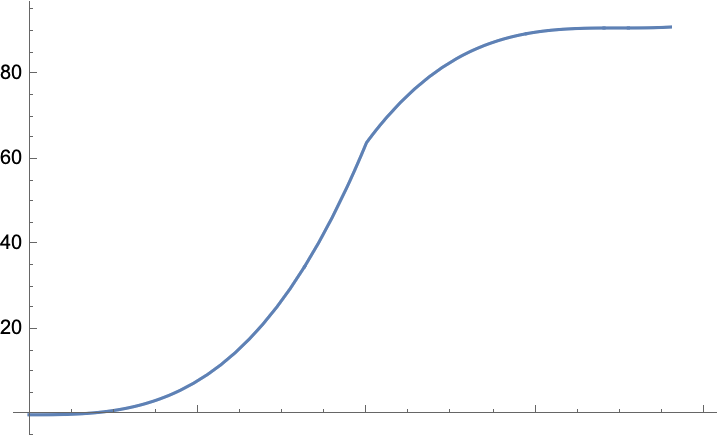
\includegraphics[width=0.3\textwidth]{score_d}
    \captionof{figure}{example curve}
    \label{fig:score_d}
\end{figure}

Money streaming is also a option to do so.

%----------------------------------------------------------------------------------------
%	REFERENCE LIST
%----------------------------------------------------------------------------------------

\begin{thebibliography}{99} % Bibliography - this is intentionally simple in this template

    \bibitem{ref1} Manu Sporny, Dave Longley, Markus Sabadello, Drummond Reed,
    Orie Steele, and Christopher Allen
    ``Decentralized Identifiers (DIDs) v1.0 Core architecture, data model, and representations''
    August 2021
    \bibitem{ref2} Parami Devs
    ``Parami Protocol Lightpaper Building Ad 3.0 For Web 3.0''
    January 2021
    \bibitem{ref3} Pascal Paillier
    ``Public-Key Cryptosystems Based on Composite Degree Residuosity Classes''
    April 1999

\end{thebibliography}

%----------------------------------------------------------------------------------------

\end{document}
